% Requires graphicx. Include in document body; hide provenance by changing
% the true switch below to false.
\newif\ifshowscriptprovenance
\showscriptprovenancetrue
\newcommand{\scriptprovenance}{%
  \ifshowscriptprovenance
  \par\noindent\textit{Script: \texttt{make\_cabmod\_figures.py}.}%
  \fi}
\begin{figure}
\centering
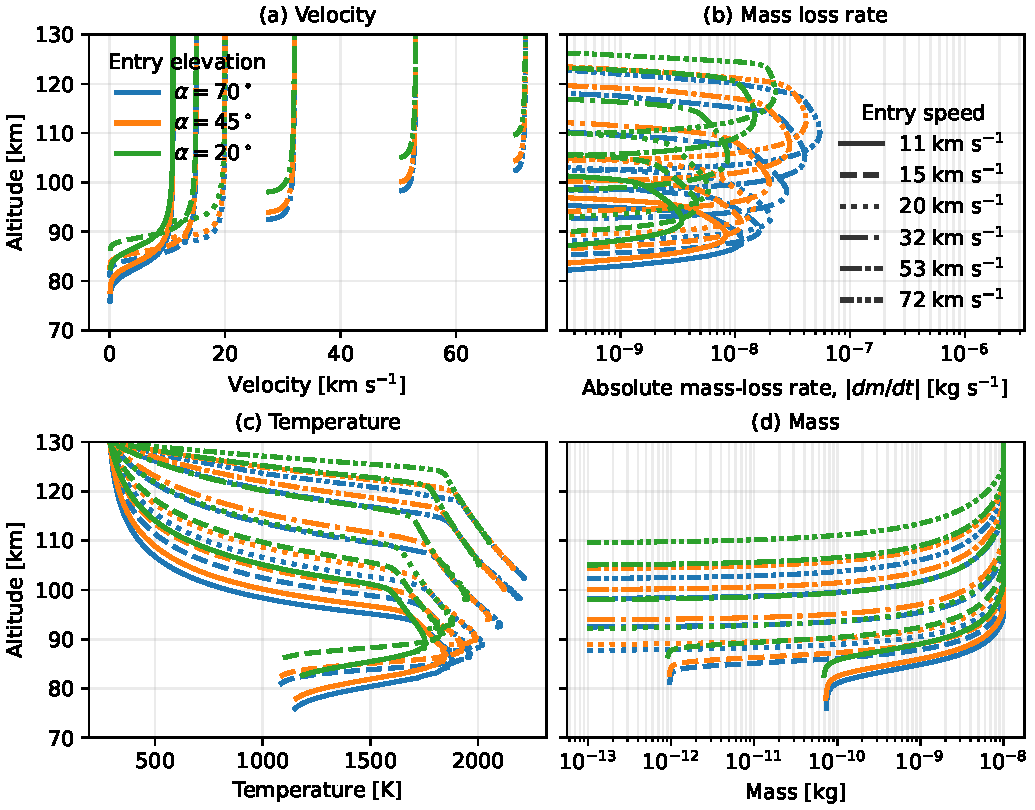
\includegraphics[width=\textwidth]{figures/meteor_ablation_single_column.pdf}
\caption{Velocity, absolute mass-loss rate, temperature, and mass versus
altitude for cometary particles of initial mass $10^{-8}$ kg. Colors denote
entry elevations $70^\circ$, $45^\circ$, and $20^\circ$; line styles denote
11, 15, 20, 32, 53, and 72 km/s.}
\scriptprovenance
\end{figure}
\begin{figure}
\centering
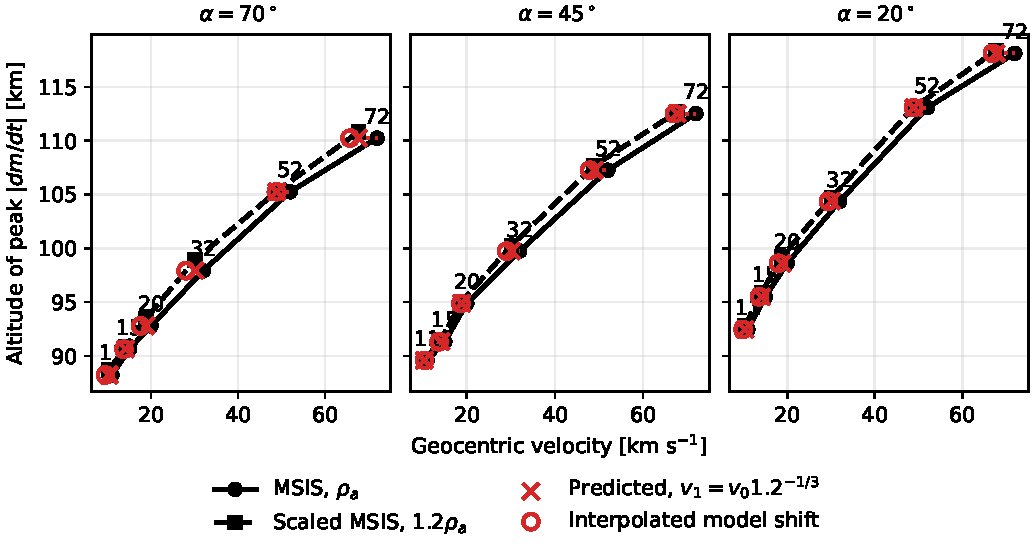
\includegraphics[width=0.99\textwidth]{figures/peak_ablation_height-1.20.pdf}
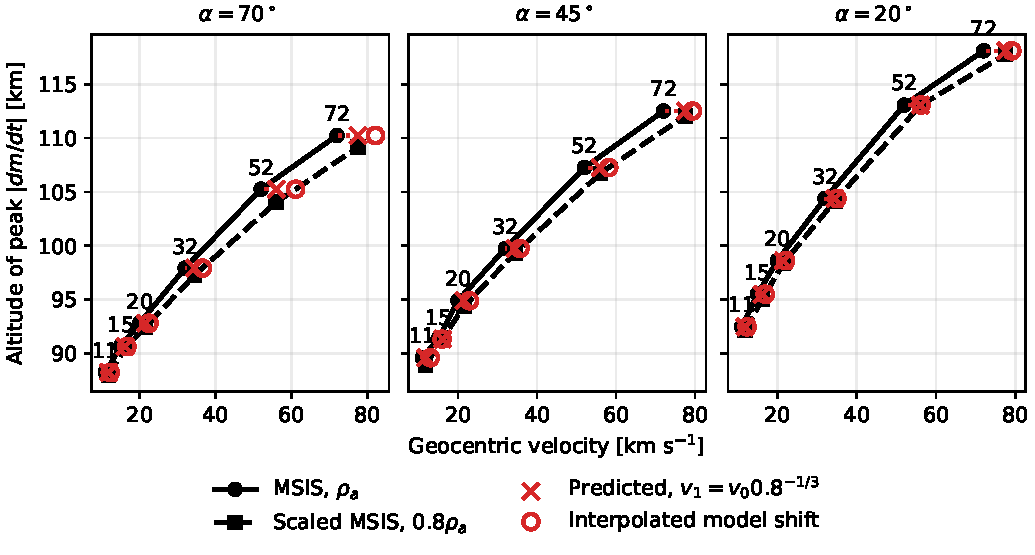
\includegraphics[width=0.99\textwidth]{figures/peak_ablation_height-0.80.pdf}
\caption{Peak mass-loss altitude versus entry speed with atmospheric density
scaled by 1.2 (top) and 0.8 (bottom). Baseline speeds are 11, 15, 20, 32, 52,
and 72 km/s. Black curves show simulations; red crosses show the
$\gamma^{-1/3}$ velocity-scaling prediction and open circles the interpolated
model shift, with linear endpoint extrapolation when needed.}
\scriptprovenance
\end{figure}
